
\subsection{Chelydridae --- Snapping Turtle}
\begin{center}
\begin{longtabu} to \textwidth {| | p{3.5cm} | X | |}

	\hline
	Taxonomy/Ancestry &
	7 extinct, 2 extant genera.
	
	\textbf{chelydra} -- 3 species native to the Americas
	
	\textbf{macrochelys} -- much larger alligator snapping turtle, 2 species exclusively N. American forming the largest freshwater turtles in N. America. A 3rd species has been proposed, the Apalachicola.
	\begin{itemize}[noitemsep]
		\item Most closely related to Platysternidae (big-headed turtles)
		\item Sometimes considered as subfamilies within the same family, but genetic evidence supports recognition as separate families
		\item Fossil record dating from Paleocene of N. America and Oligocene of Eurasia
		\item \emph{Chelydra} is known from as far back as the Pliocene in N. America
		\item \emph{Macrochelys} is known from as far as early Miocene
	\end{itemize}
	
	\begin{center} 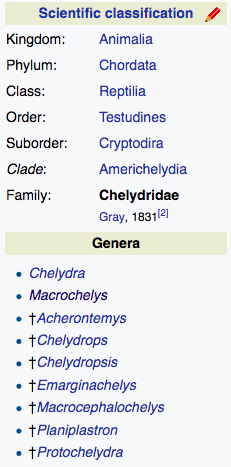
\includegraphics[scale=0.5]{testudines/chelydridae/tax} \end{center}
	 \\
	\hline
	Size & 
	7.1-31.5 in (18-80 cm); up to 249 lb (113 kg)
	\\
	\hline
	Color &
	
	 \\
	\hline
	Anatomy &
	\begin{itemize}[noitemsep]
		\item long tail
		\item 3 rows of tubercles*
		\item hooked beak
		\item kelled*, posteriorly separated carapace
		\item reduced, cruciform*, hingeless plastron
		\item heavy claws
		\item 11 marginal scutes on each side of the carapace
		\item abdominal scutes on plastron reduced; not in contact medially
		\item carapace and plastron connected by narrow bony bridge
		\item posterior skull roof deeply emancipated
	\end{itemize}
	
	The alligator snapping turtle is characterized by a large, heavy head, and a long, thick shell with three dorsal ridges of large scales (osteoderms), giving it a primitive appearance reminiscent of some of the plated dinosaurs, most notably the ankylosaurs. They can be immediately distinguished from the common snapping turtle by the three distinct rows of spikes and raised plates on the carapace, whereas the common snapping turtle has a smoother carapace. They are a solid gray, brown, black, or olive-green in color, and often covered with algae. They have radiating yellow patterns around their eyes, serving to break up the outline of the eyes to keep the turtle camouflaged. Their eyes are also surrounded by a star-shaped arrangement of fleshy, filamentous "eyelashes".
	 \\
	\hline
	Dimorphism & 
	males larger than females
	\\
	\hline
	Behavior & 
	\begin{itemize}[noitemsep]
		\item vicious temperament; since they are on top of the food chain, they have little fear
		\item snapping jaws used against prey and predators
		\item highly aquatic but leave water to nest or travel over land to reach new habitats or lay eggs
		\item diurnal, but nocturnal activity rare in northern populations
		\item most hibernate, but many individuals are capable of going w/o hibernation and remaining active beneath ice. Hibernating snapping turtles do not breathe for, in the northern part of their range, more than six months since ice covers their hibernating site. These turtles can get oxygen by pushing their head out of the mud and allowing gas exchange to take place through the membranes of their mouth and throat. This is known as extrapulmonary respiration. If they cannot get enough oxygen through this method they start to utilize anaerobic pathways, burning sugars and fats without the use of oxygen. The metabolic by-products from this process are acidic and create very undesirable side effects by spring, which are known as oxygen debt.
		\item In shallow waters, common snapping turtles may lie beneath a muddy bottom with only their heads exposed, stretching their long necks to the surface for an occasional breath (their nostrils are positioned on the very tip of the snout, effectively functioning as snorkels).
		\item Common snapping turtles sometimes bask---though rarely observed---by floating on the surface with only their carapaces exposed, though in the northern parts of their range, they also readily bask on fallen logs in early spring. 

	\end{itemize}
	\\
	\hline
	Habitat & 
	Common habitats are shallow ponds or streams. Some may inhabit brackish environments, such as estuaries. 
	\\
	\hline
	Distribution & 
	\textbf{common snapping turtle}: southeastern Canada, southwest to the edge of the Rocky Mountains, as far east as Nova Scotia and Florida.
	
	\textbf{alligator snapping turtle}: southeastern United States waters. They are found from the Florida Panhandle west to East Texas, north to southeastern Kansas, Missouri, southeastern Iowa, western Illinois, southern Wisconsin, southern Indiana, western Kentucky, and western Tennessee. They are found on the Missouri River at least as far north as the Gavins Point Dam, the southernmost dam on the Missouri River at Yankton, South Dakota, and are featured in the Gavins Point Dam Aquarium.
	
	Located from sea level to 2000 m elevation.
	\\
	\hline
	Feeding Ecology & 
	Snapping turtles consume both plant and animal matter, and are important aquatic scavengers, but they are also active hunters that prey on anything they can swallow, including many invertebrates, fish, frogs, reptiles (including snakes and smaller turtles), unwary birds, and small mammals. In some areas, adult snapping turtles can be incidentally detrimental to breeding waterfowl, as they will occasionally take ducklings and goslings but their effect on such prey is frequently exaggerated.
	
	Common snapping turtles have few predators when older, but eggs are subject to predation by crows, mink, skunks, foxes, and raccoons. As hatchlings and juveniles, most of the same predators will attack them as well as herons (mostly great blue herons), bitterns, hawks, owls, fishers, bullfrogs, large fish, and snakes. There are records during winter in Canada of hibernating adult common snapping turtles being ambushed and preyed on by northern river otters Other natural predators which have reportedly preyed on adults include coyotes, black bears, alligators and their larger cousins, alligator snapping turtles. Large, old male snapping turtles have very few natural threats due to their formidable size and defenses, and tend to have a very low annual mortality rate
	\\
	\hline
	Reproductive Biology & 
	 Courtship is variable and poorly developed and may include direct mounting, following of the female, face-offs/head-swaying, etc.
	 
	 This species mates from April through November, with their peak laying season in June and July. The female can hold sperm for several seasons, using it as necessary. Females travel over land to find sandy soil in which to lay their eggs, often some distance from the water. After digging a hole, the female typically deposits 25 to 80 hard-shelled, but not brittle eggs each year, guiding them into the nest with her hind feet and covering them with sand for incubation and protection. Incubation time is temperature-dependent, ranging from 9 to 18 weeks. In cooler climates, hatchlings overwinter in the nest. 
	 
	 TSD: intermediate temperatures produce male offspring, while high and low extremes produce females. clutches are so large that different areas of the nest may produce different sex ratios.
	 
	 Though their potential lifespans in the wild are unknown, alligator snapping turtles are believed to be capable of living to 200 years of age, but 80 to 120 is more likely. In captivity, they typically live between 20 and 70 years.
	\\
	\hline
	Ecological Role &
	have been seen as invasive species in Italy and Japan, as well as the Czech Republic and Germany for the alligator snapping turtle.
	\\
	\hline
	Conservation Status & 
	\textbf{common snapping turtle}: used as food w/ turtle soup. The species is currently classified as Least Concern by the IUCN, but has declined sufficiently due to pressure from collection for the pet trade and habitat degradation that Canada and several U.S. states have enacted or are proposing stricter conservation measures. In Canada, it is listed as 'Special Concern' in the Species at Risk Act in 2011 and is a target species for projects that include surveys, identification of major habitats, investigation and mitigation of threats, and education of the public including landowners. Involved bodies include governmental departments, universities, museums, and citizen science projects.

	\textbf{alligator snapping turtle}: Because of collection for the exotic pet trade, overharvesting for their meat, and habitat destruction, some states have imposed bans on collecting alligator snapping turtles from the wild. The IUCN lists it as a threatened species, and as of June 14, 2006, it was afforded some international protection by being listed as a CITES III species (which will put limits on exportation from the United States and all international trade in this species). The alligator snapping turtle is now endangered in several states, including Kentucky, Indiana, Illinois, and Missouri, where they are protected by state law. They are designated as ``in need of conservation" in Kansas.
	\\
	\hline
\end{longtabu}
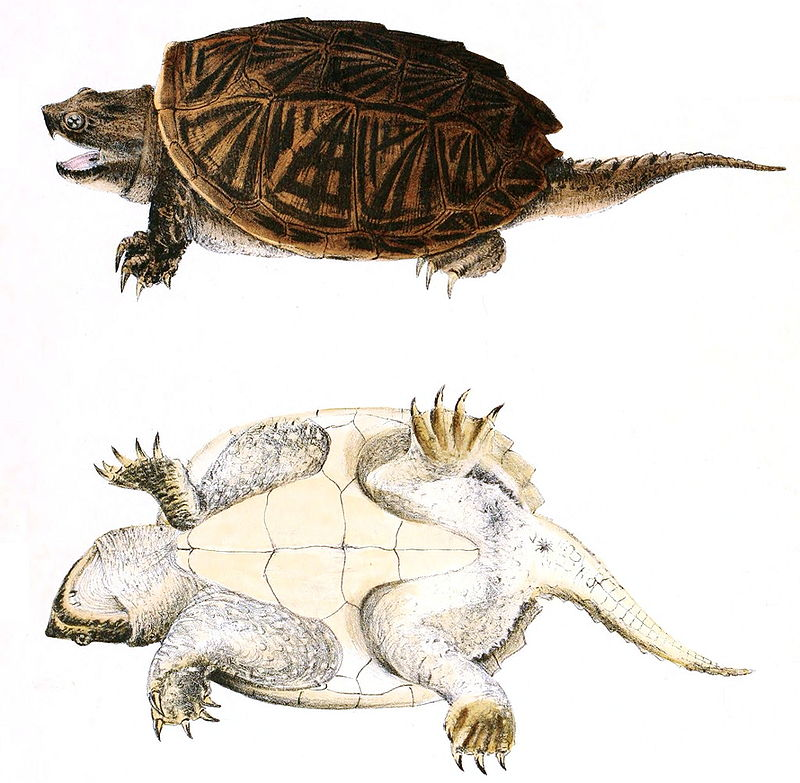
\includegraphics[scale=0.25]{testudines/chelydridae/common}
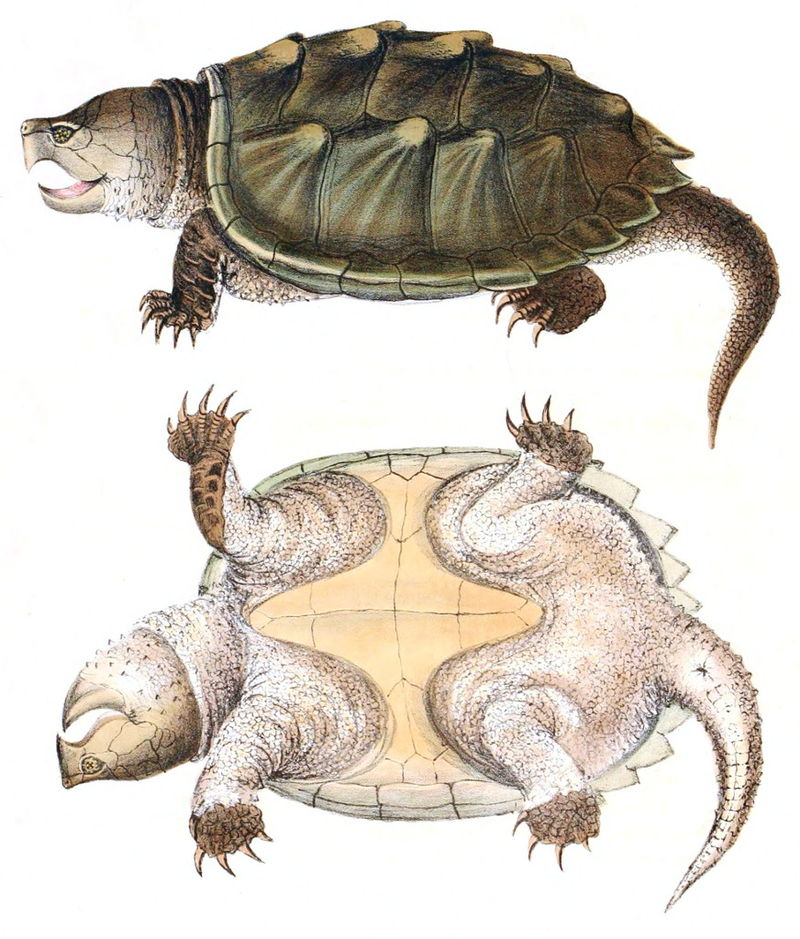
\includegraphics[scale=0.25]{testudines/chelydridae/alligator}
\end{center}